% Drawing 154/06-4 -- folder 154, batch 06, archive page 106 (PDF page 107).
% Transcription: dessins en couleur : deux paires de droites orange qui se croisent, entre elles un faisceau de droites fléchées $\lambda$, $\alpha$, $\beta$, $\gamma$, $\mu$ ; une droite vert clair et une droite en tirets, l'arc $x_0 y$ noirci ; à côté, la même configuration après une spécialisation, la droite verte passant au-dessus du premier croisement, avec les marques $x'_1 = x_0$, $y'_1 = x'$, $y'$, $z'$ et les flèches $-\lambda$, $-\alpha$, $-\beta$, $-\gamma$, $-\mu$. Plus bas, un croisement avec une bande hachurée qui s'enroule, les points $x_0$, $x$, $y$, $y'$, $z'$ ; un petit repère avec les flèches $\lambda$, $\alpha$, $\beta$, $\gamma$, $\mu$ entre $x$, $y$ et $y'$ ; et plusieurs croisements traversés de droites vert clair et de tirets bleus, avec des hachures au crayon
% Kind: pairs of crossings with a pencil of arrowed lines; specialisations; crossings with lines and dashed lines. Method 2 (schematic redraw from the facsimile). Status: partial.
% Notes: Page of colour drawings, read from the page view. Top: two pairs of orange lines crossing, between them a pencil of arrowed lines lambda, alpha, beta, gamma, mu; a light green line and a dashed line, the arc x_0 y blackened; beside it the same configuration after a specialisation, the green line passing over the first crossing (the marks x'_1 = x_0, y'_1 = x', y', z' and the arrows -lambda ... -mu are not reproduced individually). Lower: a crossing with a hatched band that winds round (points x_0, x, y', z'); a small frame with the arrows lambda ... mu between x, y and y'; and several crossings traversed by light green lines and blue dashed lines, with pencil hatching (left out); the pencilled sentences on the right are text of the transcription.
% Coordinates: 1 unit = 1 mm = 1/100 of the crop width (bbox in page fractions: [0.143, 0.108, 0.646, 0.515]).
% Redrawn by Claude (claude-opus-5-5), issue #73, 2026-11-07; not checked by a human; not compiled (no TeX in the session).
% Rights: reproduces part of the work -- behind RENDER_TRANSCRIPTS, never published by itself.
\documentclass[tikz,border=3pt]{standalone}
\usepackage{amsmath,amssymb}
\usetikzlibrary{patterns,arrows.meta}
\tikzset{Or/.style={orange!90!black}, Ye/.style={yellow!80!orange}, Lg/.style={green!60!black!70}, Dg/.style={green!45!black}, Br/.style={brown!80!black}, Rd/.style={red!85!black}, Bl/.style={blue!70!black}, Gy/.style={black!40}, pencil/.style={black!45}, struck/.style={black!35}, mark/.style={circle,draw,inner sep=1.3pt}, pt/.style={circle,fill,inner sep=0.9pt}, opt/.style={circle,draw,fill=white,inner sep=1.1pt}}
\begin{document}
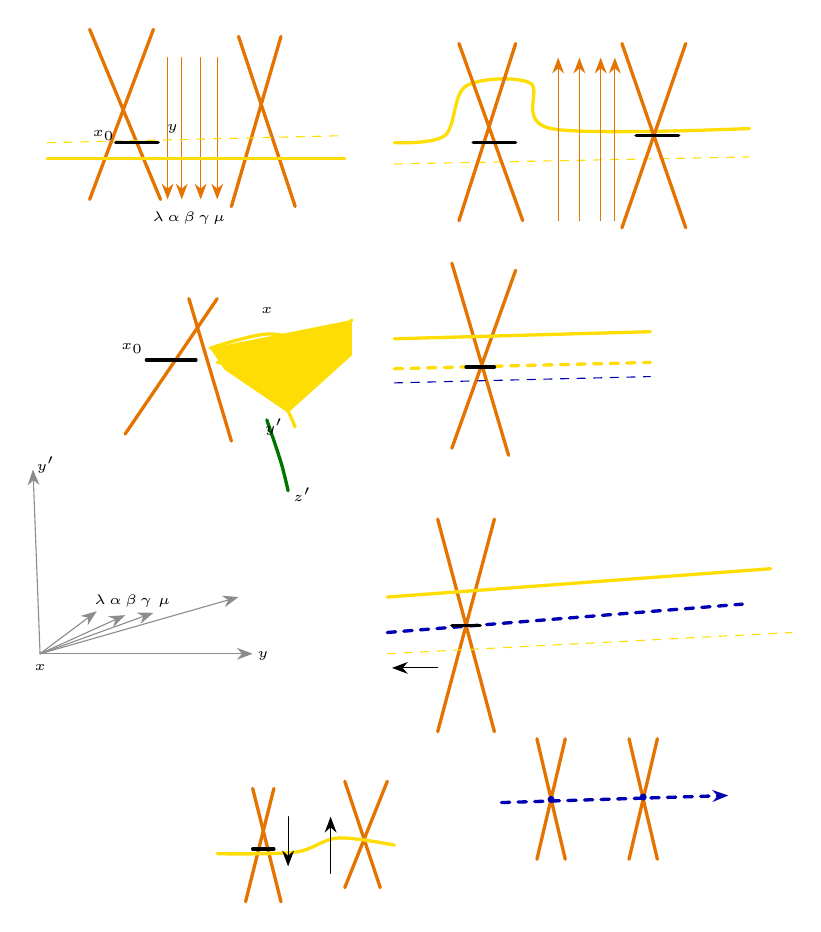
\begin{tikzpicture}[x=1mm,y=1mm,line cap=round,line join=round,font=\scriptsize]
\draw[Or,very thick] (9,-1.8) -- (18,-23.4);
\draw[Or,very thick] (17.1,-1.8) -- (9,-23.4);
\draw[Or,very thick] (27.9,-2.7) -- (35.1,-24.3);
\draw[Or,very thick] (33.3,-2.7) -- (27,-24.3);
\draw[Or,-{Stealth[length=2mm]}] (18.9,-5.4) -- (18.9,-23.4);
\draw[Or,-{Stealth[length=2mm]}] (20.7,-5.4) -- (20.7,-23.4);
\draw[Or,-{Stealth[length=2mm]}] (23.1,-5.4) -- (23.1,-23.4);
\draw[Or,-{Stealth[length=2mm]}] (25.2,-5.4) -- (25.2,-23.4);
\draw[Ye,very thick] (3.6,-18.2) -- (41.4,-18.2);
\draw[Ye,dashed] (3.6,-16.2) -- (41.4,-15.3);
\draw[very thick] (12.3,-16.2) -- (17.7,-16.2);
\node[inner sep=1pt] at (10.8,-15.3) {\tiny $x_0$};
\node[inner sep=1pt] at (19.5,-14.4) {\tiny $y$};
\node[inner sep=1pt] at (21.6,-25.8) {\tiny $\lambda\,\alpha\,\beta\,\gamma\,\mu$};
\draw[Ye,very thick] plot[smooth, tension=0.55] coordinates {(47.7,-16.2) (54.1,-15.3) (56.8,-9) (64.9,-8.6) (67.6,-14.4) (92.8,-14.4)};
\draw[Ye,dashed] (47.7,-18.9) -- (92.8,-18);
\draw[Or,very thick] (55.9,-3.6) -- (64,-26.1);
\draw[Or,very thick] (63.1,-3.6) -- (55.9,-26.1);
\draw[Or,very thick] (76.6,-3.6) -- (84.7,-27);
\draw[Or,very thick] (84.7,-3.6) -- (76.6,-27);
\draw[Or,-{Stealth[length=2mm]}] (68.5,-26.1) -- (68.5,-5.4);
\draw[Or,-{Stealth[length=2mm]}] (71.2,-26.1) -- (71.2,-5.4);
\draw[Or,-{Stealth[length=2mm]}] (73.9,-26.1) -- (73.9,-5.4);
\draw[Or,-{Stealth[length=2mm]}] (75.7,-26.1) -- (75.7,-5.4);
\draw[very thick] (57.7,-16.2) -- (63.1,-16.2);
\draw[very thick] (78.4,-15.3) -- (83.8,-15.3);
\draw[Or,very thick] (13.5,-53.2) -- (25.2,-36);
\draw[Or,very thick] (21.6,-36) -- (27,-54.1);
\draw[very thick] (16.2,-43.8) -- (22.5,-43.8);
\draw[Ye,very thick] plot[smooth, tension=0.55] coordinates {(24.3,-42.3) (31.5,-40.5) (38.7,-41.4) (42.3,-38.7)};
\draw[Ye,very thick] plot[smooth, tension=0.55] coordinates {(25.2,-44.1) (31.5,-45.9) (35.1,-52.3)};
\fill[pattern=north east lines,Ye] (24.3,-42.3) -- (42.3,-38.7) -- (42.3,-43.2) -- (34.2,-50.5) -- (26.1,-45) -- cycle;
\draw[Dg,very thick] plot[smooth, tension=0.55] coordinates {(31.5,-51.4) (33.3,-56.8) (34.2,-60.4)};
\node[inner sep=1pt] at (14.4,-42.3) {\tiny $x_0$};
\node[inner sep=1pt] at (31.5,-37.5) {\tiny $x$};
\node[inner sep=1pt] at (32.4,-52.3) {\tiny $y'$};
\node[inner sep=1pt] at (36,-60.9) {\tiny $z'$};
\draw[pencil,-{Stealth[length=2mm]}] (2.7,-81.1) -- (29.7,-81.1);
\draw[pencil,-{Stealth[length=2mm]}] (2.7,-81.1) -- (1.8,-57.7);
\draw[pencil,-{Stealth[length=2mm]}] (2.7,-81.1) -- (9.9,-75.7);
\draw[pencil,-{Stealth[length=2mm]}] (2.7,-81.1) -- (13.5,-76.2);
\draw[pencil,-{Stealth[length=2mm]}] (2.7,-81.1) -- (17.1,-75.9);
\draw[pencil,-{Stealth[length=2mm]}] (2.7,-81.1) -- (27.9,-73.9);
\node[inner sep=1pt] at (14.4,-74.4) {\tiny $\lambda\,\alpha\,\beta\,\gamma\ \mu$};
\node[inner sep=1pt] at (2.7,-82.9) {\tiny $x$};
\node[inner sep=1pt] at (31,-81.4) {\tiny $y$};
\node[inner sep=1pt] at (3.4,-57.1) {\tiny $y'$};
\draw[Or,very thick] (55,-31.5) -- (62.2,-55.9);
\draw[Or,very thick] (63.1,-32.4) -- (55,-55);
\draw[Ye,very thick] (47.7,-41.1) -- (80.2,-40.2);
\draw[Ye,dashed,very thick] (47.7,-44.9) -- (80.2,-44.1);
\draw[Bl,dashed] (47.7,-46.7) -- (80.2,-45.9);
\draw[very thick] (56.8,-44.7) -- (60.4,-44.7);
\draw[Or,very thick] (53.2,-64) -- (60.4,-91);
\draw[Or,very thick] (60.4,-64) -- (53.2,-91);
\draw[Ye,very thick] (46.8,-73.9) -- (95.5,-70.3);
\draw[Bl,dashed,very thick] (46.8,-78.4) -- (91.9,-74.8);
\draw[Ye,dashed] (46.8,-81.1) -- (98.2,-78.4);
\draw[very thick] (55,-77.5) -- (58.6,-77.5);
\draw[-{Stealth[length=2mm]}] (53.2,-82.9) -- (47.4,-82.9);
\draw[Or,very thick] (29.7,-98.2) -- (33.3,-112.6);
\draw[Or,very thick] (32.4,-98.2) -- (28.8,-112.6);
\draw[Or,very thick] (41.4,-97.3) -- (45.9,-110.8);
\draw[Or,very thick] (46.8,-97.3) -- (41.4,-110.8);
\draw[Ye,very thick] plot[smooth, tension=0.55] coordinates {(25.2,-106.5) (35.1,-106.3) (40.5,-104.5) (47.7,-105.4)};
\draw[-{Stealth[length=2mm]}] (34.2,-101.8) -- (34.2,-108.1);
\draw[-{Stealth[length=2mm]}] (39.6,-109) -- (39.6,-101.8);
\draw[very thick] (29.7,-105.9) -- (32.4,-105.9);
\draw[Or,very thick] (65.8,-91.9) -- (69.4,-107.2);
\draw[Or,very thick] (69.4,-91.9) -- (65.8,-107.2);
\draw[Or,very thick] (77.5,-91.9) -- (81.1,-107.2);
\draw[Or,very thick] (81.1,-91.9) -- (77.5,-107.2);
\draw[Bl,dashed,very thick,-{Stealth[length=2mm]}] (61.3,-100) -- (90.1,-99.1);
\node[pt,Bl] at (67.6,-99.6) {};
\node[pt,Bl] at (79.3,-99.3) {};
\end{tikzpicture}
\end{document}
